% answers.tex —— 2010 年·春季上海卷 · 参考答案与详细解析片段
% 由 tools/generate_projects.py 依来源总账自 2010/2010_数学真题_春季上海_试题.md + 2010/2010_数学真题_春季上海_解析正文.md + 2010/2010_数学真题_春季上海_答案要点.md 生成，勿手改（改源 MD 后重跑）


\begin{gktip}
以下推导仅依据固定 PDF 第 1–2 页题面独立写出，再与第 3–4 页印载的“参考答案”逐题对照；两处一致处不再另注，不一致或需说明处标【源疑点】。固定副本是《数学教学》2010 年第 2 期转载版（印刷页 2-37 至 2-40），其出版者、版次与官方身份未核实，故本稿不称“官方解析”。分数、根号、上下标与选项均按 600 dpi 原页复核。
\end{gktip}

\begin{answer}
\gksolhead{1}{}

\textbf{题目}：

函数 $y=\dfrac12\sin 2x$ 的最小正周期 $T=$ $\underline{\qquad}$。

\Needspace{4\baselineskip}
\textbf{解析}
\Needspace{5\baselineskip}
形如 $y=A\sin\omega x$ 的函数，最小正周期为 $T=\dfrac{2\pi}{|\omega|}$。此处 $A=\dfrac12$，$\omega=2$，振幅不影响周期，故
\nopagebreak[4]
\[T=\frac{2\pi}{2}=\pi.\]
\Needspace{5\baselineskip}
验证最小性：若 $T>0$ 使 $\sin(2x+2T)=\sin2x$ 对一切 $x$ 成立，则
\nopagebreak[4]
\[\sin(2x+2T)-\sin2x=2\cos(2x+T)\sin T\equiv0,\]
取使 $\cos(2x+T)\neq0$ 的 $x$ 得 $\sin T=0$，即 $T=k\pi\ (k\in\mathbf N^*)$，最小正值 $T=\pi$，与上式一致。

\gkanswer{答案：$\pi$。}

\end{answer}
\begin{answer}
\gksolhead{2}{}

\textbf{题目}：

已知函数 $f(x)=ax^2+2x$ 是奇函数，则实数 $a=$ $\underline{\qquad}$。

\Needspace{4\baselineskip}
\textbf{解析}
\Needspace{5\baselineskip}
$f(x)$ 为奇函数，即对一切实数 $x$ 有 $f(-x)=-f(x)$：
\nopagebreak[4]
\[ax^2-2x=-\left(ax^2+2x\right)=-ax^2-2x.\]
两边消去 $-2x$ 得 $2ax^2=0$ 对一切 $x$ 成立，故 $a=0$。
代回验证：$a=0$ 时 $f(x)=2x$，$f(-x)=-2x=-f(x)$，确为奇函数。
另用单点检验：$f(1)=a+2$，$-f(-1)=-(a-2)=2-a$，令二者相等也得 $a=0$，与上面一致。

\gkanswer{答案：$0$。}

\end{answer}
\begin{answer}
\gksolhead{3}{}

\textbf{题目}：

计算：$\dfrac{2\mathrm i}{1+\mathrm i}=$ $\underline{\qquad}$（$\mathrm i$ 为虚数单位）。

\Needspace{4\baselineskip}
\textbf{解析}
\Needspace{5\baselineskip}
分子分母同乘 $1-\mathrm i$：
\nopagebreak[4]
\[\frac{2\mathrm i}{1+\mathrm i}=\frac{2\mathrm i\left(1-\mathrm i\right)}{\left(1+\mathrm i\right)\left(1-\mathrm i\right)}=\frac{2\mathrm i-2\mathrm i^2}{1+1}=\frac{2+2\mathrm i}{2}=1+\mathrm i.\]
代回验证：$(1+\mathrm i)^2=1+2\mathrm i+\mathrm i^2=2\mathrm i$，与被除数相同，结果正确。

\gkanswer{答案：$1+\mathrm i$。}

\end{answer}
\begin{answer}
\gksolhead{4}{}

\textbf{题目}：

已知集合 $A=\{x\mid |x|<2\}$，$B=\left\{x\mid \dfrac{1}{x+1}>0\right\}$，则 $A\cap B=$ $\underline{\qquad}$。

\Needspace{4\baselineskip}
\textbf{解析}
由 $|x|<2$ 得 $A=(-2,2)$。
\Needspace{5\baselineskip}
集合 $B$ 中分子恒为 $1>0$，故
\nopagebreak[4]
\[\frac{1}{x+1}>0\iff x+1>0\iff x>-1,\]
\Needspace{5\baselineskip}
即 $B=(-1,+\infty)$。于是
\nopagebreak[4]
\[A\cap B=(-2,2)\cap(-1,+\infty)=(-1,2),\]
写成描述法即 $\{x\mid -1<x<2\}$。
代回检验：$x=0$ 满足 $|0|<2$ 且 $\dfrac1{0+1}=1>0$，在交集中；$x=-\dfrac32$ 只属于 $A$；$x=2$ 不属于 $A$（$|2|<2$ 不成立），也不属于交集，端点开闭与 $(-1,2)$ 相符。

\gkanswer{答案：$\{x\mid -1<x<2\}$（即 $(-1,2)$）。}

\end{answer}
\begin{answer}
\gksolhead{5}{}

\textbf{题目}：

若椭圆 $\dfrac{x^2}{25}+\dfrac{y^2}{16}=1$ 上一点 $P$ 到焦点 $F_1$ 的距离为 $6$，则点 $P$ 到另一个焦点 $F_2$ 的距离是 $\underline{\qquad}$。

\Needspace{4\baselineskip}
\textbf{解析}
\Needspace{5\baselineskip}
椭圆 $\dfrac{x^2}{25}+\dfrac{y^2}{16}=1$ 中 $a^2=25$，$a=5$，故
\nopagebreak[4]
\[|PF_1|+|PF_2|=2a=10.\]
已知 $|PF_1|=6$，于是 $|PF_2|=10-6=4$。
合理性检验：$c=\sqrt{25-16}=3$，椭圆上点到焦点的距离落在 $[a-c,a+c]=[2,8]$ 内，$4$ 在其中，且 $P$ 存在（以 $F_2$ 为圆心、$4$ 为半径的圆与椭圆有交点）。

\gkanswer{答案：$4$。}

\end{answer}
\begin{answer}
\gksolhead{6}{}

\textbf{题目}：

某社区对居民进行上海世博会知晓情况的分层抽样调查。已知该社区有青年人、中年人和老年人分别有 $800$ 人、$1600$ 人、$1400$ 人。若在老年人中的抽样人数是 $70$，则在中年人中的抽样人数应该是 $\underline{\qquad}$。

\Needspace{4\baselineskip}
\textbf{解析}
\Needspace{5\baselineskip}
分层抽样按比例抽取。老年人 $1400$ 人中抽 $70$ 人，抽样比为
\nopagebreak[4]
\[\frac{70}{1400}=\frac1{20}.\]
\Needspace{5\baselineskip}
中年人 $1600$ 人，应抽
\nopagebreak[4]
\[\frac{1600}{20}=80\ \text{\text{人}}.\]
整体校验：青年人应抽 $\dfrac{800}{20}=40$ 人，合计 $40+80+70=190$，而全社区 $800+1600+1400=3800$，$3800\times\dfrac1{20}=190$，比例一致。

\gkanswer{答案：$80$。}

\end{answer}
\begin{answer}
\gksolhead{7}{}

\textbf{题目}：

已知双曲线 $C$ 经过点 $(1,1)$，它的一条渐近线方程为 $y=\sqrt3x$，则双曲线 $C$ 的标准方程是 $\underline{\qquad}$。

\Needspace{4\baselineskip}
\textbf{解析}
\Needspace{5\baselineskip}
若双曲线焦点在 $x$ 轴上，标准形式为 $\dfrac{x^2}{a^2}-\dfrac{y^2}{b^2}=1$，渐近线为 $y=\pm\dfrac ba x$。由 $y=\sqrt3x$ 得
\nopagebreak[4]
\[\frac{b}{a}=\sqrt3,\qquad b^2=3a^2.\]
\Needspace{5\baselineskip}
代入点 $(1,1)$：
\nopagebreak[4]
\[\frac1{a^2}-\frac1{b^2}=1\iff\frac1{a^2}-\frac1{3a^2}=1\iff\frac{2}{3a^2}=1\iff a^2=\frac23,\]
\Needspace{5\baselineskip}
从而 $b^2=3\times\dfrac23=2$，方程为
\nopagebreak[4]
\[\frac{x^2}{2/3}-\frac{y^2}{2}=1.\]
排除另一种定向：若焦点在 $y$ 轴，方程为 $\dfrac{y^2}{a^2}-\dfrac{x^2}{b^2}=1$，渐近线 $y=\pm\dfrac ab x$ 给出 $a^2=3b^2$，代入 $(1,1)$ 得 $\dfrac1{3b^2}-\dfrac1{b^2}=-\dfrac{2}{3b^2}=1$，无正数解，故不可能。
代回验证：$\dfrac{1}{2/3}-\dfrac12=\dfrac32-\dfrac12=1$，点在曲线上；$\dfrac{x^2}{2/3}-\dfrac{y^2}{2}=0\iff y^2=3x^2$，渐近线正是 $y=\pm\sqrt3x$，含 $y=\sqrt3x$。

\gkanswer{答案：$\dfrac{x^2}{2/3}-\dfrac{y^2}{2}=1$。}

\end{answer}
\begin{answer}
\gksolhead{8}{}

\textbf{题目}：

在 $\left(2x^2+\dfrac1x\right)^6$ 的二项展开式中，常数项是 $\underline{\qquad}$。

\Needspace{4\baselineskip}
\textbf{解析}
\Needspace{5\baselineskip}
二项展开式的通项为
\nopagebreak[4]
\[T_{k+1}=\mathrm C_6^k\left(2x^2\right)^{6-k}\left(\frac1x\right)^k=\mathrm C_6^k2^{6-k}x^{12-2k-k}=\mathrm C_6^k2^{6-k}x^{12-3k},\quad k=0,1,\dots,6.\]
\Needspace{5\baselineskip}
常数项要求 $x$ 的指数为零：
\nopagebreak[4]
\[12-3k=0\iff k=4.\]
\Needspace{5\baselineskip}
故常数项为
\nopagebreak[4]
\[\mathrm C_6^4\cdot2^{6-4}=15\times4=60.\]
核对相邻项：$k=3$ 时指数为 $3$，$k=5$ 时指数为 $-3$，均非常数项，$k=4$ 是唯一解。

\gkanswer{答案：$60$。}

\end{answer}
\begin{answer}
\gksolhead{9}{}

\textbf{题目}：

连续掷两次骰子，出现点数之和等于 $4$ 的概率为 $\underline{\qquad}$（结果用数值表示）。

\Needspace{4\baselineskip}
\textbf{解析}
两次掷骰的结果组成有序对 $(i,j)$，$i,j\in\{1,2,\dots,6\}$，共 $6\times6=36$ 个等可能基本事件，每个概率为 $\dfrac1{36}$。
\Needspace{5\baselineskip}
点数和为 $4$ 的有序对只有三个：
\nopagebreak[4]
\[(1,3),\quad(2,2),\quad(3,1).\]
（$i\ge1$、$j\ge1$，故 $(4,0)$、$(0,4)$ 之类不出现，和为 $4$ 的情形恰好这三种。）
\Needspace{5\baselineskip}
逐个计算各基本事件的概率再相加：
\nopagebreak[4]
\[P=\frac1{36}+\frac1{36}+\frac1{36}=\frac3{36}=\frac1{12}.\]
复核：把 $36$ 种情形中点和为 $4$ 的个数直接数出亦为 $3$，与上面一致。

\gkanswer{答案：$\dfrac1{12}$。}

\end{answer}
\begin{answer}
\gksolhead{10}{}

\textbf{题目}：

各棱长都为 $1$ 的正四棱锥的体积 $V=$ $\underline{\qquad}$。

\Needspace{4\baselineskip}
\textbf{解析}
正四棱锥底面是边长为 $1$ 的正方形，侧棱长也为 $1$。设底面中心为 $O'$，顶点为 $P$，则 $P$ 在过 $O'$ 且垂直于底面的直线上。
\Needspace{5\baselineskip}
底面正方形对角线长为 $\sqrt2$，$O'$ 到顶点 $A$ 的距离为 $\dfrac{\sqrt2}{2}$。在直角三角形 $PO'A$ 中
\nopagebreak[4]
\[PO'=\sqrt{PA^2-O'A^2}=\sqrt{1-\left(\frac{\sqrt2}{2}\right)^2}=\sqrt{\frac12}=\frac{\sqrt2}{2}.\]
\Needspace{5\baselineskip}
底面积 $S=1$，故
\nopagebreak[4]
\[V=\frac13Sh=\frac13\times1\times\frac{\sqrt2}{2}=\frac{\sqrt2}{6}.\]
量纲与量级检验：边长 $1$ 的正方体体积为 $1$，该锥高约 $0.707$、底面积 $1$，体积约 $0.236$，与 $\dfrac{\sqrt2}{6}\approx0.2357$ 相符。

\gkanswer{答案：$\dfrac{\sqrt2}{6}$。}

\end{answer}
\begin{answer}
\gksolhead{11}{}

\textbf{题目}：

方程 $\begin{vmatrix}1&2&4\\1&x&x^2\\1&-3&9\end{vmatrix}=0$ 的解集为 $\underline{\qquad}$。

\Needspace{4\baselineskip}
\textbf{解析}
\Needspace{5\baselineskip}
按第一行展开三阶行列式：
\nopagebreak[4]
\[\begin{vmatrix}1&2&4\\1&x&x^2\\1&-3&9\end{vmatrix}
=1\cdot\left(9x+3x^2\right)-2\cdot\left(9-x^2\right)+4\cdot\left(-3-x\right).\]
\Needspace{5\baselineskip}
逐项化简：
\nopagebreak[4]
\[9x+3x^2-18+2x^2-12-4x=5x^2+5x-30=5\left(x+3\right)\left(x-2\right).\]
方程为 $5(x+3)(x-2)=0$，故 $x=-3$ 或 $x=2$，解集为 $\{-3,2\}$。
代回验证：$x=2$ 时第二行为 $(1,2,4)$，与第一行相同，行列式为 $0$；$x=-3$ 时第二行为 $(1,-3,9)$，与第三行相同，行列式为 $0$。二次方程至多两个实根，故解集不再有其他元素。

\gkanswer{答案：$\{-3,2\}$。}

\end{answer}
\begin{answer}
\gksolhead{12}{}

\textbf{题目}：

根据所示的程序框图（其中 $[x]$ 表示不大于 $x$ 的最大整数），输出 $r=$ $\underline{\qquad}$。
\nopagebreak[4]
\begin{center}% 2010 年上海春季卷第 12 题：程序框图。
% 来源 PDF：春季高考/2010/2010春季上海.pdf，SHA-256 24926e5272a6316cbaa399c0a097b3986ab34563db975016f98bae99f2274c56。
% 原页：第 1 页右栏下部（印刷页 2-37，《数学教学》2010 年第 2 期转载）。
% 重绘依据：开始 → a←√5，b←√7，n←1 → 判断 n(b−a)>1；否则 n←n+1 回到判断；
% 是则 m←[na] → r←(m+1)/n → 输出 r → 结束。循环回线接在判断框上方。
\begin{tikzpicture}[semithick, every node/.style={inner sep=2pt, font=\small}, >=stealth]
  \node[draw, rounded corners] (start) at (0,0) {开始};
  \node[draw, rectangle] (init) at (0,-1.2) {$a\leftarrow\sqrt5,\ b\leftarrow\sqrt7,\ n\leftarrow1$};
  \node[draw, diamond, aspect=2.4] (test) at (0,-3.0) {$n(b-a)>1$};
  \node[draw, rectangle] (inc) at (2.9,-3.0) {$n\leftarrow n+1$};
  \node[draw, rectangle] (m) at (0,-4.4) {$m\leftarrow[na]$};
  \node[draw, rectangle] (r) at (0,-5.4) {$r\leftarrow(m+1)/n$};
  \node[draw, trapezium, trapezium left angle=70, trapezium right angle=110] (out) at (0,-6.5) {输出 $r$};
  \node[draw, rounded corners] (end) at (0,-7.6) {结束};

  \draw[->] (start) -- (init);
  \draw[->] (init) -- (test);
  \draw[->] (test) -- node[above] {否} (inc);
  \draw[->] (inc.north) -- (2.9,-2.05) -- (0,-2.05);
  \draw[->] (0,-2.05) -- (test.north);
  \draw[->] (test) -- node[right] {是} (m);
  \draw[->] (m) -- (r);
  \draw[->] (r) -- (out);
  \draw[->] (out) -- (end);
\end{tikzpicture}
\end{center}
\nopagebreak[4]
\Needspace{4\baselineskip}
\textbf{解析}
\Needspace{5\baselineskip}
先算常数：$a=\sqrt5\approx2.236068$，$b=\sqrt7\approx2.645751$，
\nopagebreak[4]
\[b-a\approx0.409683.\]
判断框为 $n(b-a)>1$，$n$ 从 $1$ 起逐个增加：

\begin{itemize}
\item $n=1$：$0.409683<1$，取“否”分支，$n\leftarrow2$；
\item $n=2$：$2\times0.409683=0.819366<1$，$n\leftarrow3$；
\item $n=3$：$3\times0.409683=1.229049>1$，取“是”分支，退出循环。
\end{itemize}

\Needspace{5\baselineskip}
于是 $n=3$，$m=[na]=[3\sqrt5]$。因 $3\sqrt5\approx6.708204$，故
\nopagebreak[4]
\[m=[6.708204]=6.\]
\Needspace{5\baselineskip}
最后
\nopagebreak[4]
\[r=\frac{m+1}{n}=\frac{6+1}{3}=\frac73.\]
边界核对：$[3\sqrt5]=7$ 需要 $3\sqrt5\ge7$，即 $45\ge49$，不成立，故取整确为 $6$，不是 $7$。

\gkanswer{答案：$\dfrac73$。}

\end{answer}
\begin{answer}
\gksolhead{13}{}

\textbf{题目}：

在下图所示的斜截圆柱中，已知圆柱底面的直径为 $40\,\mathrm{cm}$，母线长最短 $50\,\mathrm{cm}$、最长 $80\,\mathrm{cm}$，则斜截圆柱侧面面积 $S=$ $\underline{\qquad}$ $\mathrm{cm}^2$。
\nopagebreak[4]
\begin{center}% 2010 年上海春季卷第 13 题：斜截圆柱示意（底面直径 40 cm，母线最短 50 cm、最长 80 cm）。
% 来源 PDF：春季高考/2010/2010春季上海.pdf，SHA-256 24926e5272a6316cbaa399c0a097b3986ab34563db975016f98bae99f2274c56。
% 原页：第 1 页右栏中部（印刷页 2-37，《数学教学》2010 年第 2 期转载）。
% 重绘依据：圆柱下底为椭圆（上沿虚线、下沿实线），底面直径标 40 cm；
% 截口为倾斜椭圆，左母线 50 cm、右母线 80 cm 用双向箭头标注。
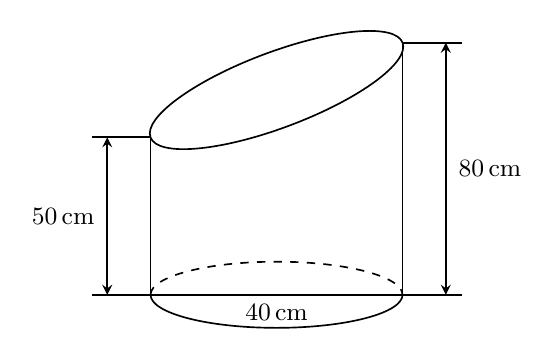
\begin{tikzpicture}[semithick, every node/.style={inner sep=1.5pt, font=\small}, >=stealth]
  % 下底椭圆：上半（背面）虚线，下半（正面）实线
  \draw[dashed] (-1.6,0) arc[start angle=180, end angle=0, x radius=1.6, y radius=0.42];
  \draw (-1.6,0) arc[start angle=180, end angle=360, x radius=1.6, y radius=0.42];
  % 底面直径
  \draw (-1.6,0) -- (1.6,0);
  \node at (0,-0.22) {$40\,\mathrm{cm}$};
  % 两条母线
  \draw (-1.6,0) -- (-1.6,2.0);
  \draw (1.6,0) -- (1.6,3.2);
  % 截口椭圆：两端点恰为两条母线的上端点 (-1.6,2.0) 与 (1.6,3.2)
  \draw[rotate around={20.6:(0,2.6)}] (0,2.6) ellipse (1.71 and 0.48);
  % 左侧 50 cm 标注
  \draw (-1.6,0) -- (-2.35,0);
  \draw (-1.6,2.0) -- (-2.35,2.0);
  \draw[<->] (-2.15,0) -- (-2.15,2.0);
  \node[left] at (-2.25,1.0) {$50\,\mathrm{cm}$};
  % 右侧 80 cm 标注
  \draw (1.6,0) -- (2.35,0);
  \draw (1.6,3.2) -- (2.35,3.2);
  \draw[<->] (2.15,0) -- (2.15,3.2);
  \node[right] at (2.25,1.6) {$80\,\mathrm{cm}$};
\end{tikzpicture}
\end{center}
\nopagebreak[4]
\Needspace{4\baselineskip}
\textbf{解析}
沿一条母线把侧面剪开铺平。斜截圆柱的侧面展开后，是一块上下两边平行、下边为直线（底面圆周展开成的线段，长 $2\pi r=40\pi$）、上边为斜直线（截口展开）的图形，母线长从左到右由 $50$ 线性增到 $80$。
\Needspace{5\baselineskip}
设展开后横向坐标为 $u\in[0,2\pi]$，母线长为
\nopagebreak[4]
\[h(u)=65-15\cos u,\]
\Needspace{5\baselineskip}
其平均值
\nopagebreak[4]
\[\frac1{2\pi}\int_0^{2\pi}h(u)\,\mathrm du=65-\frac{15}{2\pi}\int_0^{2\pi}\cos u\,\mathrm du=65.\]
\Needspace{5\baselineskip}
侧面积等于“横向弧长元 $r\,\mathrm du$”与母线长之积的积分：
\nopagebreak[4]
\[S=\int_0^{2\pi}h(u)\,r\,\mathrm du=r\int_0^{2\pi}\left(65-15\cos u\right)\mathrm du=20\times65\times2\pi=2600\pi.\]
即 $S=$（底面周长）$\times$（平均母线长）$=40\pi\times65=2600\pi\approx8168\ \mathrm{cm}^2$。
合理性检验：若按直圆柱粗估，取平均母线 $65$，侧面积 $40\pi\times65$；母线的长短相对 $65$ 的偏差正负相消，故结果与“周长 × 平均母线长”一致。

\gkanswer{答案：$2600\pi$。}

\end{answer}
\begin{answer}
\gksolhead{14}{}

\textbf{题目}：

\Needspace{5\baselineskip}
设 $n$ 阶方阵
\nopagebreak[4]
\[A_n=\begin{pmatrix}
1&3&5&\cdots&2n-1\\
2n+1&2n+3&2n+5&\cdots&4n-1\\
4n+1&4n+3&4n+5&\cdots&6n-1\\
\vdots&\vdots&\vdots&&\vdots\\
2n(n-1)+1&2n(n-1)+3&2n(n-1)+5&\cdots&2n^2-1
\end{pmatrix}.\]
任取 $A_n$ 中的一个元素，记为 $x_1$；划去 $x_1$ 所在的行和列，将剩下的元素按原来的位置关系组成 $n-1$ 阶方阵 $A_{n-1}$，任取 $A_{n-1}$ 中的一个元素，记为 $x_2$；划去 $x_2$ 所在的行和列，$\cdots\cdots$；将最后剩下的一个元素记为 $x_n$。记 $S_n=x_1+x_2+\cdots+x_n$，则 $\lim\limits_{n\to\infty}\dfrac{S_n}{n^3+1}=$ $\underline{\qquad}$。

\Needspace{4\baselineskip}
\textbf{解析}
\Needspace{5\baselineskip}
先写出 $A_n$ 的通项。第 $i$ 行首个元素为 $2n(i-1)+1$，同行逐列加 $2$，故
\nopagebreak[4]
\[a_{ij}=2n\left(i-1\right)+\left(2j-1\right),\qquad 1\le i,j\le n.\]
（核对：$i=1$ 给 $1,3,5,\dots,2n-1$；$i=2$ 给 $2n+1,\dots,4n-1$；$i=n$ 给 $2n(n-1)+1,\dots,2n^2-1$，与原页相符。）
\Needspace{5\baselineskip}
抽取过程中，每次划去一行一列，故第 $k$ 次取到的元素 $x_k=a_{i_kj_k}$ 中的 $i_1,i_2,\dots,i_n$ 互不相同、恰为 $1,2,\dots,n$ 的一个排列，$j_1,\dots,j_n$ 亦然。于是
\nopagebreak[4]
\[S_n=\sum_{k=1}^{n}\left[2n\left(i_k-1\right)+\left(2j_k-1\right)\right]
=2n\sum_{k=1}^{n}\left(i_k-1\right)+\sum_{k=1}^{n}\left(2j_k-1\right).\]
\Needspace{5\baselineskip}
两个和都与排列无关：
\nopagebreak[4]
\[\sum_{k=1}^{n}\left(i_k-1\right)=\sum_{i=1}^{n}\left(i-1\right)=\frac{n(n-1)}{2},\qquad
\sum_{k=1}^{n}\left(2j_k-1\right)=\sum_{j=1}^{n}\left(2j-1\right)=n^2.\]
\Needspace{5\baselineskip}
故
\nopagebreak[4]
\[S_n=2n\cdot\frac{n(n-1)}{2}+n^2=n^2(n-1)+n^2=n^3,\]
\Needspace{5\baselineskip}
与每次具体取哪个元素无关。于是
\nopagebreak[4]
\[\lim_{n\to\infty}\frac{S_n}{n^3+1}=\lim_{n\to\infty}\frac{n^3}{n^3+1}=1.\]
小规模核对：$n=1$ 时 $A_1=(1)$，$S_1=1=1^3$；$n=2$ 时 $A_2=\begin{pmatrix}1&3\\5&7\end{pmatrix}$，三种取法分别得 $1+7=8$、$3+5=8$、$5+3=8$，均为 $2^3=8$，与公式一致。

\gkanswer{答案：$1$。}

\end{answer}
\begin{answer}
\gksolhead{15}{}

\textbf{题目}：

若空间三条直线 $a$、$b$、$c$ 满足 $a\perp b$，$b\perp c$，则直线 $a$ 与 $c$　[答]（　）

（A）一定平行。

（B）一定相交。

（C）一定是异面直线。

（D）平行、相交、是异面直线都有可能。

\Needspace{4\baselineskip}
\textbf{解析}
取 $b$ 为 $z$ 轴，则 $a\perp b$、$c\perp b$ 表示 $a$、$c$ 的方向向量都平行于 $xOy$ 平面。三种位置都可能出现：

\begin{itemize}
\item 平行：取 $a$、$c$ 方向相同且分处不同高度，二者平行；
\item 相交：在同一点处作两条都垂直于 $b$ 且方向不同的直线，二者相交；
\item 异面：在 $z=0$ 与 $z=1$ 两个水平面内各取一条方向不同的直线，二者不平行也不相交，是异面直线。
\end{itemize}
逐项排除：（A）“一定平行”被相交之例否定；（B）“一定相交”被平行之例否定；（C）“一定是异面直线”被相交之例否定；（D）与三例都相容。
故选 D。

\gkanswer{答案：D。}

\end{answer}
\begin{answer}
\gksolhead{16}{}

\textbf{题目}：

已知 $a_1$、$a_2\in(0,1)$。记 $M=a_1a_2$，$N=a_1+a_2-1$，则 $M$ 与 $N$ 的大小关系是　[答]（　）

（A）$M<N$。

（B）$M>N$。

（C）$M=N$。

（D）不确定。

\Needspace{4\baselineskip}
\textbf{解析}
\Needspace{5\baselineskip}
作差：
\nopagebreak[4]
\[M-N=a_1a_2-\left(a_1+a_2-1\right)=a_1a_2-a_1-a_2+1=\left(1-a_1\right)\left(1-a_2\right).\]
因 $a_1,a_2\in(0,1)$，有 $1-a_1>0$、$1-a_2>0$，故 $(1-a_1)(1-a_2)>0$，即 $M>N$ 恒成立。
数值检验：取 $a_1=a_2=\dfrac12$，$M=\dfrac14$，$N=0$，$M>N$；取 $a_1=0.1$、$a_2=0.9$，$M=0.09$，$N=0$，仍 $M>N$；取 $a_1=a_2=0.9$，$M=0.81$，$N=0.8$，仍 $M>N$。
逐项排除：（A）$M<N$ 与上式相反；（C）$M=N$ 需 $(1-a_1)(1-a_2)=0$，与 $a_1,a_2\in(0,1)$ 矛盾；（D）“不确定”被 $M>N$ 恒成立否定。
故选 B。

\gkanswer{答案：B。}

\end{answer}
\begin{answer}
\gksolhead{17}{}

\textbf{题目}：

已知抛物线 $C:y^2=x$ 与直线 $l:y=kx+1$。“$k\neq0$”是“直线 $l$ 与抛物线 $C$ 有两个不同的交点”的　[答]（　）

（A）充分不必要条件。

（B）必要不充分条件。

（C）充要条件。

（D）既不充分也不必要条件。

\Needspace{4\baselineskip}
\textbf{解析}
\Needspace{5\baselineskip}
把 $y=kx+1$ 代入 $y^2=x$：
\nopagebreak[4]
\[\left(kx+1\right)^2=x\iff k^2x^2+\left(2k-1\right)x+1=0.\quad(\ast)\]
讨论 $k$ 的取值：

\begin{itemize}
\item $k=0$ 时 $(\ast)$ 退化为 $-x+1=0$，即 $x=1$，直线 $y=1$ 与抛物线只有一个交点 $(1,1)$。
\item $k\neq0$ 时 $(\ast)$ 是二次方程，两交点不同等价于判别式为正：
\end{itemize}
\nopagebreak[4]
\[\Delta=\left(2k-1\right)^2-4k^2=1-4k>0\iff k<\frac14.\]
故“$k\neq0$”是“有两个不同交点”的必要条件（$k=0$ 时只有一个交点），但不充分：例如 $k=1$ 满足 $k\neq0$，而 $\Delta=1-4=-3<0$，直线与抛物线无交点；$k=\dfrac12$ 时 $\Delta=-1<0$，同样无交点。
逐项排除：（A）把必要说成充分；（C）充要需两边等价，而 $k<\dfrac14$ 与 $k\neq0$ 并不等价；（D）否定了确实成立的必要性。
故选 B。

\gkanswer{答案：B。}

\end{answer}
\begin{answer}
\gksolhead{18}{}

\textbf{题目}：

已知函数 $f(x)=\dfrac{1}{4-2^x}$ 的图像关于点 $P$ 对称，则点 $P$ 的坐标是　[答]（　）

（A）$\left(2,\dfrac12\right)$。

（B）$\left(2,\dfrac14\right)$。

（C）$\left(2,\dfrac18\right)$。

（D）$(0,0)$。

\Needspace{4\baselineskip}
\textbf{解析}
先定对称中心的横坐标。$4-2^x=0\iff x=2$，$x=2$ 是唯一竖直渐近线；当 $x\to2^-$ 时 $4-2^x\to0^+$，$f(x)\to+\infty$，当 $x\to2^+$ 时 $f(x)\to-\infty$。若图像关于点 $(a,b)$ 中心对称，则渐近线 $x=2$ 必须映为自身，故 $a=2$。
\Needspace{5\baselineskip}
再定纵坐标。设 $P=(2,b)$，中心对称要求
\nopagebreak[4]
\[f(2+h)+f(2-h)=2b\quad\text{\text{对一切} }h\neq0\text{ \text{成立}}.\]
\Needspace{5\baselineskip}
记 $u=2^h>0$，则
\nopagebreak[4]
\[f(2+h)=\frac1{4-4\cdot2^h}=\frac1{4(1-u)},\qquad f(2-h)=\frac1{4-4\cdot2^{-h}}=\frac1{4\left(1-\frac1u\right)}=\frac{u}{4(u-1)},\]
\Needspace{5\baselineskip}
两式相加：
\nopagebreak[4]
\[f(2+h)+f(2-h)=\frac14\left[\frac1{1-u}+\frac{u}{u-1}\right]=\frac14\cdot\frac{1-u}{1-u}=\frac14.\]
故 $2b=\dfrac14$，$b=\dfrac18$，即 $P\left(2,\dfrac18\right)$。
逐项排除：（A）$\left(2,\dfrac12\right)$ 要求两对称点和为 $1$，实际和为 $\dfrac14$；（B）$\left(2,\dfrac14\right)$ 要求和为 $\dfrac12$；（D）关于原点对称要求 $f(-x)=-f(x)$，但 $f(0)=\dfrac13$，不满足 $f(0)=0$。
故选 C。

\gkanswer{答案：C。}

\end{answer}
\begin{answer}
\gksolhead{19}{}

\textbf{题目}（本题满分 12 分）：

已知 $\tan\theta=a\ (a>1)$，求 $\dfrac{\sin\left(\dfrac\pi4+\theta\right)}{\sin\left(\dfrac\pi2-\theta\right)}\cdot\tan2\theta$ 的值。

\Needspace{4\baselineskip}
\textbf{解析}
由 $\tan\theta=a>1$ 知 $\theta$ 在第一或第三象限（模 $\pi$），故 $\cos\theta\neq0$；又 $a>1$ 使 $1-\tan^2\theta\neq0$，各步变形都有意义。
\Needspace{5\baselineskip}
先化简两个三角比：
\nopagebreak[4]
\[\sin\left(\frac\pi2-\theta\right)=\cos\theta,\qquad
\sin\left(\frac\pi4+\theta\right)=\sin\frac\pi4\cos\theta+\cos\frac\pi4\sin\theta=\frac{\sqrt2}{2}\left(\sin\theta+\cos\theta\right),\]
\Needspace{5\baselineskip}
故
\nopagebreak[4]
\[\frac{\sin\left(\frac\pi4+\theta\right)}{\sin\left(\frac\pi2-\theta\right)}
=\frac{\frac{\sqrt2}{2}\left(\sin\theta+\cos\theta\right)}{\cos\theta}
=\frac{\sqrt2}{2}\left(1+\tan\theta\right)=\frac{\sqrt2}{2}\left(1+a\right).\]
\Needspace{5\baselineskip}
再由二倍角公式
\nopagebreak[4]
\[\tan2\theta=\frac{2\tan\theta}{1-\tan^2\theta}=\frac{2a}{1-a^2}.\]
\Needspace{5\baselineskip}
相乘：
\nopagebreak[4]
\[\frac{\sqrt2}{2}\left(1+a\right)\cdot\frac{2a}{1-a^2}
=\frac{\sqrt2}{2}\left(1+a\right)\cdot\frac{2a}{\left(1-a\right)\left(1+a\right)}
=\frac{\sqrt2a}{1-a}.\]
【源疑点】卷内解题末步的分母印作 $1-a$（$600$ dpi 下可辨，非 $1-a^2$），与本推导一致；扫描件中该处的上标易误读为平方，特此说明。
\Needspace{5\baselineskip}
数值检验：取 $a=2$（即 $\tan\theta=2$，$\sin\theta=\dfrac{2}{\sqrt5}$，$\cos\theta=\dfrac1{\sqrt5}$），
\nopagebreak[4]
\[\frac{\sin\left(\frac\pi4+\theta\right)}{\cos\theta}=\frac{\frac{\sqrt2}{2}\cdot\frac{3}{\sqrt5}}{\frac1{\sqrt5}}=\frac{3\sqrt2}{2},\qquad \tan2\theta=\frac{4}{1-4}=-\frac43,\]
乘积为 $\dfrac{3\sqrt2}{2}\times\left(-\dfrac43\right)=-2\sqrt2$，而 $\dfrac{\sqrt2\times2}{1-2}=-2\sqrt2$，相符。

\gkanswer{答案：$\dfrac{\sqrt2a}{1-a}$。}

\end{answer}
\begin{answer}
\gksolhead{20}{}

\textbf{题目}（本题满分 14 分）本题共有 2 个小题，第 1 小题满分 6 分，第 2 小题满分 8 分。：

已知函数 $f(x)=\log_a(8-2^x)$（$a>0$，且 $a\neq1$）。

（1）若函数 $f(x)$ 的反函数是其本身，求 $a$ 的值；

（2）当 $a>1$ 时，求函数 $y=f(x)+f(-x)$ 的最大值。

\Needspace{4\baselineskip}
\textbf{解析}
\Needspace{5\baselineskip}
（1）先求反函数。由 $y=\log_a\left(8-2^x\right)$ 得 $a^y=8-2^x$，即 $2^x=8-a^y$，故
\nopagebreak[4]
\[x=\log_2\left(8-a^y\right),\qquad f^{-1}(x)=\log_2\left(8-a^x\right).\]
\Needspace{5\baselineskip}
“反函数是其本身”要求 $f(x)=f^{-1}(x)$ 在公共定义域上恒成立：
\nopagebreak[4]
\[\log_a\left(8-2^x\right)=\log_2\left(8-a^x\right).\]
\Needspace{5\baselineskip}
取 $x=0$（此时 $8-2^0=7>0$，$8-a^0=7>0$，两边都有意义）：
\nopagebreak[4]
\[\log_a7=\log_27\iff a=2.\]
代回验证：$a=2$ 时左右两端都等于 $\log_2\left(8-2^x\right)$，恒等成立。故 $a=2$，且由 $x=0$ 处的取值唯一确定。

（2）先定定义域：$8-2^x>0$ 且 $8-2^{-x}>0$，即 $2^x<8$ 且 $2^{-x}<8$，解得 $-3<x<3$。
\Needspace{5\baselineskip}
在 $(-3,3)$ 上，
\nopagebreak[4]
\[y=f(x)+f(-x)=\log_a\left(8-2^x\right)+\log_a\left(8-2^{-x}\right)=\log_a\left[\left(8-2^x\right)\left(8-2^{-x}\right)\right].\]
\Needspace{5\baselineskip}
展开括号：
\nopagebreak[4]
\[\left(8-2^x\right)\left(8-2^{-x}\right)=64-8\cdot2^{-x}-8\cdot2^x+1=65-8\left(2^x+2^{-x}\right).\]
由均值不等式 $2^x+2^{-x}\ge2\sqrt{2^x\cdot2^{-x}}=2$，等号当且仅当 $2^x=2^{-x}$，即 $x=0$。
\Needspace{5\baselineskip}
于是
\nopagebreak[4]
\[0<65-8\left(2^x+2^{-x}\right)\le65-16=49,\]
左端严格为正是因为在 $(-3,3)$ 内 $2^x+2^{-x}<\dfrac{65}{8}=8.125$（端点处趋于该值）。
\Needspace{5\baselineskip}
当 $a>1$ 时 $\log_a t$ 关于 $t$ 单调递增，故
\nopagebreak[4]
\[y\le\log_a49,\]
等号在 $x=0$ 处取得。所求最大值为 $\log_a49$。
检验：$x=0$ 时 $y=2\log_a7=\log_a49$，与上式一致；$x\to\pm3$ 时 $65-8\left(2^x+2^{-x}\right)\to0^+$，$y\to-\infty$，说明最大值确实在内部取得。

\gkanswer{答案：（1）$a=2$；（2）最大值为 $\log_a 49$（当 $x=0$ 时取得）。}

\end{answer}
\begin{answer}
\gksolhead{21}{}

\textbf{题目}（本题满分 14 分）本题共有 2 个小题，第 1 小题满分 6 分，第 2 小题满分 8 分。：

已知地球的半径约为 $6371$ 千米。上海的位置约为东经 $121^\circ$、北纬 $31^\circ$，大连的位置为东经 $121^\circ$、北纬 $39^\circ$，里斯本的位置约为西经 $10^\circ$、北纬 $39^\circ$。

（1）若飞机以平均速度 $720$ 千米/小时飞行，则从上海到大连的最短飞行时间约为多少小时（飞机飞行高度忽略不计，结果精确到 $0.1$ 小时）？

（2）求大连与里斯本之间的球面距离（结果精确到 $1$ 千米）。
\nopagebreak[4]
\begin{center}% 2010 年上海春季卷第 21 题：地球示意图（北极—南极、赤道、上海/大连所在经线与纬线、里斯本）。
% 来源 PDF：春季高考/2010/2010春季上海.pdf，SHA-256 24926e5272a6316cbaa399c0a097b3986ab34563db975016f98bae99f2274c56。
% 原页：第 2 页右栏中部（印刷页 2-38，《数学教学》2010 年第 2 期转载）。
% 重绘依据：球面轮廓 + 地轴虚线；北纬 39° 圈（实线）过大连、里斯本；
% 北纬 31° 圈（虚线）过上海；南侧另有赤道圈（实线）；经线用椭圆弧表示，
% 大连与上海同在东经 121° 经线上。
\begin{tikzpicture}[semithick, every node/.style={inner sep=1.5pt, font=\small}]
  % 球面轮廓与地轴
  \draw (0,0) circle (2);
  \draw[dashed] (0,2) -- (0,-2);
  % 纬圈：北纬 39°（实线，过大连、里斯本）
  \draw (0,1.15) ellipse (1.55 and 0.30);
  % 纬圈：北纬 31°（虚线，过上海）
  \draw[dashed] (0,0.66) ellipse (1.72 and 0.33);
  % 赤道（实线，位于视点下方）
  \draw (0,-0.45) ellipse (1.94 and 0.38);
  % 经线：左前方一条（实线）、过上海与大连一条（实线）、近中央背面一条（虚线）
  \draw (0,2) arc[start angle=90, end angle=270, x radius=0.55, y radius=2];
  \draw (0,2) arc[start angle=90, end angle=-90, x radius=0.735, y radius=2];
  \draw[dashed] (0,2) arc[start angle=90, end angle=-90, x radius=0.40, y radius=2];
  % 三地位置
  \fill (-1.55,1.15) circle (1.6pt);
  \node[left] at (-1.60,1.15) {里斯本};
  \fill (0.655,0.878) circle (1.6pt);
  \node at (0.60,1.15) {大连};
  \fill (0.727,0.361) circle (1.6pt);
  \node[right] at (0.755,0.361) {上海};
  % 球心与两极
  \node at (0.20,-0.10) {$O$};
  \node[above] at (0,2.05) {北极};
  \node[below] at (0,-2.05) {南极};
\end{tikzpicture}
\end{center}
\nopagebreak[4]
\Needspace{4\baselineskip}
\textbf{解析}
\Needspace{5\baselineskip}
（1）上海（东经 $121^\circ$、北纬 $31^\circ$）与大连（东经 $121^\circ$、北纬 $39^\circ$）在同一经线上，故同在一个大圆（经线圈）上，最短航线即该大圆的劣弧。球心角等于纬度差
\nopagebreak[4]
\[\angle AOB=39^\circ-31^\circ=8^\circ=\frac{8\pi}{180}\ \text{rad}.\]
\Needspace{5\baselineskip}
弧长（球面距离）
\nopagebreak[4]
\[l=6371\times\frac{8\pi}{180}\approx6371\times0.139626\approx889.56\ \text{\text{千米}}.\]
\Needspace{5\baselineskip}
飞行时间
\nopagebreak[4]
\[t=\frac{889.56}{720}\approx1.236\ \text{\text{小时}},\]
精确到 $0.1$ 小时为 $1.2$ 小时。
量级检验：赤道一周约 $4.0\times10^4$ 千米，$8^\circ$ 约占 $\dfrac8{360}$，即约 $890$ 千米，与上面一致。

\Needspace{5\baselineskip}
（2）记球心为 $O$，大连为 $B$（北纬 $39^\circ$、东经 $121^\circ$），里斯本为 $C$（北纬 $39^\circ$、西经 $10^\circ$）。两地纬度相同，经度差
\nopagebreak[4]
\[\Delta\lambda=121^\circ-\left(-10^\circ\right)=131^\circ.\]
\Needspace{5\baselineskip}
以球心为原点、地轴为 $z$ 轴建系，单位球面上
\nopagebreak[4]
\[\begin{aligned}
B&=\left(\cos39^\circ\cos121^\circ,\ \cos39^\circ\sin121^\circ,\ \sin39^\circ\right),\\
C&=\left(\cos39^\circ\cos\left(-10^\circ\right),\ \cos39^\circ\sin\left(-10^\circ\right),\ \sin39^\circ\right).
\end{aligned}\]
\Needspace{5\baselineskip}
由数量积
\nopagebreak[4]
\[\cos\angle BOC=\sin^239^\circ+\cos^239^\circ\cos131^\circ.\]
\Needspace{5\baselineskip}
代入 $\sin39^\circ\approx0.629320$，$\cos39^\circ\approx0.777146$，$\cos131^\circ\approx-0.656059$：
\nopagebreak[4]
\[\cos\angle BOC\approx0.396044+0.603956\times\left(-0.656059\right)\approx0.396044-0.396230\approx-1.87\times10^{-4}.\]
\Needspace{5\baselineskip}
故
\nopagebreak[4]
\[\angle BOC=\arccos\left(-1.87\times10^{-4}\right)\approx90.011^\circ,\]
\Needspace{5\baselineskip}
球面距离
\nopagebreak[4]
\[s=6371\times\frac{90.011\pi}{180}\approx6371\times1.570993\approx10009\ \text{\text{千米}}.\]
\Needspace{5\baselineskip}
交叉核对（同纬度小圆法）：北纬 $39^\circ$ 圈的半径为 $r\cos39^\circ$，弦长
\nopagebreak[4]
\[BC=2r\cos39^\circ\sin\frac{131^\circ}{2}=2\times6371\times0.777146\times\sin65.5^\circ\approx9011\ \text{\text{千米}},\]
由 $\sin\dfrac{\angle BOC}{2}=\dfrac{BC}{2r}=\cos39^\circ\sin65.5^\circ\approx0.707166$ 得 $\dfrac{\angle BOC}{2}\approx45.007^\circ$，即 $\angle BOC\approx90.01^\circ$，与上面一致。
【源疑点】卷内解答用“过 $B$ 作与赤道平面平行的截面”的余弦定理算法，得 $\angle BOC\approx90.01^\circ$、球面距离约 $10009$ 千米；本稿用球面余弦定理独立算出同一结果（未四舍五入前约 $10008.8$ 千米），两者不矛盾。

\gkanswer{答案：（1）约 $1.2$ 小时；（2）约 $10009$ 千米。}

\end{answer}
\begin{answer}
\gksolhead{22}{}

\textbf{题目}（本题满分 16 分）本题共有 3 个小题，第 1 小题满分 4 分，第 2 小题满分 6 分，第 3 小题满分 6 分。：

在平面上，给定非零向量 $\vec b$。对任意向量 $\vec a$，定义 $\vec a'=\vec a-\dfrac{2\left(\vec a\cdot\vec b\right)}{\left|\vec b\right|^2}\vec b$。

（1）若 $\vec a=(2,3)$，$\vec b=(-1,3)$，求 $\vec a'$；

（2）若 $\vec b=(2,1)$，证明：若位置向量 $\vec a$ 的终点在直线 $Ax+By+C=0$ 上，则位置向量 $\vec a'$ 的终点也在一条直线上；

（3）已知存在单位向量 $\vec b$，当位置向量 $\vec a$ 的终点在抛物线 $C:x^2=y$ 上时，位置向量 $\vec a'$ 的终点总在抛物线 $C':y^2=x$ 上。曲线 $C$ 与 $C'$ 关于直线 $l$ 对称，问直线 $l$ 与向量 $\vec b$ 满足什么关系？

\Needspace{4\baselineskip}
\textbf{解析}
\Needspace{5\baselineskip}
（1）$\vec a=(2,3)$，$\vec b=(-1,3)$，则
\nopagebreak[4]
\[\vec a\cdot\vec b=2\times(-1)+3\times3=7,\qquad\left|\vec b\right|^2=(-1)^2+3^2=10.\]
\Needspace{5\baselineskip}
故
\nopagebreak[4]
\[\vec a'=(2,3)-\frac{2\times7}{10}(-1,3)=(2,3)-\frac75(-1,3)=\left(2+\frac75,\ 3-\frac{21}{5}\right)=\left(\frac{17}{5},-\frac65\right).\]
检验：$\vec a'\cdot\vec b=\dfrac{17}{5}\times(-1)+\left(-\dfrac65\right)\times3=-\dfrac{17}{5}-\dfrac{18}{5}=-7=-\vec a\cdot\vec b$，即 $\vec a'$ 是 $\vec a$ 关于 $\vec b$ 的垂线的对称向量，符合定义中“反射”的特征。

\Needspace{5\baselineskip}
（2）$\vec b=(2,1)$，$\left|\vec b\right|^2=5$，$\vec a\cdot\vec b=2x+y$，故
\nopagebreak[4]
\[\begin{aligned}
\vec a'&=(x,y)-\frac{2(2x+y)}5(2,1)\\
&=\left(x-\frac{4(2x+y)}5,\ y-\frac{2(2x+y)}5\right)\\
&=\left(-\frac35x-\frac45y,\ -\frac45x+\frac35y\right).
\end{aligned}\]
\Needspace{5\baselineskip}
记 $\vec a'=(x',y')$，写成矩阵形式
\nopagebreak[4]
\[\begin{pmatrix}x'\\y'\end{pmatrix}=\frac15\begin{pmatrix}-3&-4\\-4&3\end{pmatrix}\begin{pmatrix}x\\y\end{pmatrix}.\]
\Needspace{5\baselineskip}
该矩阵满足 $M^2=I$（直接验算：$\dfrac1{25}\begin{pmatrix}9+16&12-12\\12-12&16+9\end{pmatrix}=I$），故逆变换就是它本身：
\nopagebreak[4]
\[x=-\frac35x'-\frac45y',\qquad y=-\frac45x'+\frac35y'.\]
（这与“关于直线 $2x+y=0$ 的对称”一致：该直线正是 $\vec b$ 的垂线。）
\Needspace{5\baselineskip}
把上式代入 $Ax+By+C=0$：
\nopagebreak[4]
\[A\left(-\frac35x'-\frac45y'\right)+B\left(-\frac45x'+\frac35y'\right)+C=0,\]
\Needspace{5\baselineskip}
整理得
\nopagebreak[4]
\[-\frac15\left(3A+4B\right)x'+\frac15\left(-4A+3B\right)y'+C=0.\quad(\ast)\]
\Needspace{5\baselineskip}
还需说明 $(\ast)$ 确为一条直线，即两个系数不同时为零。若
\nopagebreak[4]
\[3A+4B=0\quad\text{\text{且}}\quad-4A+3B=0,\]
则由第一式 $3A=-4B$，代入第二式得 $-4A+3\cdot\left(-\dfrac{3A}{4}\right)=0$，即 $-\dfrac{25}{4}A=0$，故 $A=0$，进而 $B=0$，与“$A$、$B$ 不全为零”矛盾。于是 $(\ast)$ 是直线方程，$\vec a'$ 的终点在该直线上。

\Needspace{5\baselineskip}
（3）设 $\vec b=(b_1,b_2)$，由 $\left|\vec b\right|=1$ 得 $b_1^2+b_2^2=1$。曲线 $C:x^2=y$ 上的点可写作 $\vec a=(t,t^2)$（$t\in\mathbf R$），于是
\nopagebreak[4]
\[\vec a\cdot\vec b=tb_1+t^2b_2,\]
\nopagebreak[4]
\[\vec a'=(t,t^2)-2\left(tb_1+t^2b_2\right)(b_1,b_2)
=\left(t-2b_1^2t-2b_1b_2t^2,\ t^2-2b_1b_2t-2b_2^2t^2\right),\]
\Needspace{5\baselineskip}
即
\nopagebreak[4]
\[\vec a'=\left(\left(1-2b_1^2\right)t-2b_1b_2t^2,\ -2b_1b_2t+\left(1-2b_2^2\right)t^2\right).\]
\Needspace{5\baselineskip}
题设要求 $\vec a'$ 的终点恒在 $C':y^2=x$ 上，即对一切 $t$
\nopagebreak[4]
\[\left[-2b_1b_2t+\left(1-2b_2^2\right)t^2\right]^2=\left(1-2b_1^2\right)t-2b_1b_2t^2.\quad(\star)\]
\Needspace{5\baselineskip}
左端是关于 $t$ 的至多四次式，其 $t^4$ 项系数为 $\left(1-2b_2^2\right)^2$；右端是至多二次式。恒等式要求四次项系数为零：
\nopagebreak[4]
\[\left(1-2b_2^2\right)^2=0\iff b_2^2=\frac12.\]
此时左端 $=t^2\cdot\left(-2b_1b_2\right)^2=4b_1^2b_2^2t^2$，再由 $b_1^2+b_2^2=1$ 得 $b_1^2=\dfrac12$，故 $4b_1^2b_2^2=4\times\dfrac12\times\dfrac12=1$。
\Needspace{5\baselineskip}
回到 $(\star)$，比较 $t$ 与 $t^2$ 的系数：
\nopagebreak[4]
\[1-2b_1^2=0\ (\text{\text{已满足}}),\qquad 1=-2b_1b_2\iff b_1b_2=-\frac12<0.\]
\Needspace{5\baselineskip}
结合 $b_1^2=b_2^2=\dfrac12$ 与 $b_1b_2<0$，得
\nopagebreak[4]
\[\vec b=\pm\left(\frac{\sqrt2}{2},-\frac{\sqrt2}{2}\right).\]
\Needspace{5\baselineskip}
题中又给出 $C:x^2=y$ 与 $C':y^2=x$ 关于直线 $l$ 对称，而这两条抛物线关于直线 $y=x$ 对称，故 $l:y=x$，其方向向量 $\vec d=(1,1)$。计算
\nopagebreak[4]
\[\vec d\cdot\vec b=1\cdot\left(\pm\frac{\sqrt2}{2}\right)+1\cdot\left(\mp\frac{\sqrt2}{2}\right)=0,\]
故 $\vec d\perp\vec b$，即直线 $l$ 与向量 $\vec b$ 垂直。
\Needspace{5\baselineskip}
检验：取 $\vec b=\left(\dfrac{\sqrt2}{2},-\dfrac{\sqrt2}{2}\right)$，则 $\vec a'$ 的两坐标为
\nopagebreak[4]
\[x'=\left(1-2\cdot\frac12\right)t-2\cdot\left(-\frac12\right)t^2=t^2,\qquad y'=-2\cdot\left(-\frac12\right)t+\left(1-2\cdot\frac12\right)t^2=t,\]
恰为 $(t^2,t)$，满足 $y'^2=t^2=x'$，即点 $\vec a'$ 在 $C':y^2=x$ 上，与题设相符。

\gkanswer{答案：（1）$\left(\dfrac{17}{5},-\dfrac65\right)$；（2）$\vec a'$ 的终点在直线 $-\dfrac15(3A+4B)x+\dfrac15(-4A+3B)y+C=0$ 上；（3）$l\perp\vec b$，且 $\vec b=\pm\left(\dfrac{\sqrt2}{2},-\dfrac{\sqrt2}{2}\right)$。}

\end{answer}
\begin{answer}
\gksolhead{23}{}

\textbf{题目}（本题满分 18 分）本题共有 3 个小题，第 1 小题满分 4 分，第 2 小题满分 6 分，第 3 小题满分 8 分。：

已知首项为 $x_1$ 的数列 $\{x_n\}$ 满足 $x_{n+1}=\dfrac{ax_n}{x_n+1}$（$a$ 为常数）。

（1）若对任意的 $x_1\neq-1$，有 $x_{n+2}=x_n$ 对任意的 $n\in\mathbf N^*$ 都成立，求 $a$ 的值；

（2）当 $a=1$ 时，若 $x_1>0$，数列 $\{x_n\}$ 是递增数列还是递减数列？请说明理由；

（3）当 $a$ 确定后，数列 $\{x_n\}$ 由其首项 $x_1$ 确定。当 $a=2$ 时，通过对数列 $\{x_n\}$ 的探究，写出“$\{x_n\}$ 是有穷数列”的一个真命题（不必证明）。

说明：对于第（3）题，将根据写出真命题所体现的思维层次和对问题探究的完整性，给予不同的评分。

\Needspace{4\baselineskip}
\textbf{解析}
\Needspace{5\baselineskip}
（1）反复用递推式：
\nopagebreak[4]
\[x_{n+2}=\frac{ax_{n+1}}{x_{n+1}+1}=\frac{a\cdot\dfrac{ax_n}{x_n+1}}{\dfrac{ax_n}{x_n+1}+1}=\frac{a^2x_n}{ax_n+x_n+1}=\frac{a^2x_n}{\left(a+1\right)x_n+1}.\]
\Needspace{5\baselineskip}
要求 $x_{n+2}=x_n$ 对一切 $x_1\neq-1$、一切 $n\in\mathbf N^*$ 成立。取 $n=1$，此时 $x_n=x_1$ 可取任意 $\neq-1$ 的实数，故对一切这样的 $x_1$（并使分母不为零）
\nopagebreak[4]
\[\frac{a^2x_1}{\left(a+1\right)x_1+1}=x_1.\]
\Needspace{5\baselineskip}
两边乘以 $\left(a+1\right)x_1+1$，得
\nopagebreak[4]
\[a^2x_1=\left[\left(a+1\right)x_1+1\right]x_1\iff\left(a+1\right)x_1^2+\left(1-a^2\right)x_1=0.\]
\Needspace{5\baselineskip}
右式是关于 $x_1$ 的多项式，它在无穷多个 $x_1$ 上取零，故恒等于零：
\nopagebreak[4]
\[\left(a+1\right)x^2+\left(1-a^2\right)x\equiv0.\]
比较系数得 $a+1=0$ 且 $1-a^2=0$，故 $a=-1$。
\Needspace{5\baselineskip}
代回验证：$a=-1$ 时 $x_{n+1}=-\dfrac{x_n}{x_n+1}$，于是
\nopagebreak[4]
\[x_{n+2}=-\frac{x_{n+1}}{x_{n+1}+1}=-\frac{-\frac{x_n}{x_n+1}}{-\frac{x_n}{x_n+1}+1}=\frac{\frac{x_n}{x_n+1}}{\frac{1}{x_n+1}}=x_n,\]
确为周期 $2$ 的循环。

（2）当 $a=1$ 时 $x_{n+1}=\dfrac{x_n}{x_n+1}$。由 $x_1>0$ 归纳：若 $x_n>0$，则 $x_{n+1}=\dfrac{x_n}{x_n+1}>0$，故一切 $x_n>0$。
\Needspace{5\baselineskip}
作差：
\nopagebreak[4]
\[x_{n+1}-x_n=\frac{x_n}{x_n+1}-x_n=\frac{x_n-x_n\left(x_n+1\right)}{x_n+1}=\frac{-x_n^2}{x_n+1}<0,\]
因 $x_n>0$ 使分母为正、分子为负。故 $\{x_n\}$ 是递减数列。
补充：$x_n>0$ 且递减，故有下界 $0$，必有极限；设极限为 $L\ge0$，得 $L=\dfrac{L}{L+1}$，即 $L=0$，与“递减”相容（例如 $x_1=1$ 时 $x_n=\dfrac1n$）。

（3）当 $a=2$ 时 $x_{n+1}=\dfrac{2x_n}{x_n+1}$。若某项 $x_n=-1$，则 $x_{n+1}$ 的分母为零，递推中断，数列到此为止，共 $n$ 项。故“有穷”等价于存在 $n$ 使 $x_n=-1$。
\Needspace{5\baselineskip}
令 $y_n=\dfrac1{x_n}$（只要 $x_n\neq0$），则
\nopagebreak[4]
\[y_{n+1}=\frac{x_n+1}{2x_n}=\frac12+\frac12y_n,\]
\Needspace{5\baselineskip}
即 $y_{n+1}-1=\dfrac12\left(y_n-1\right)$，故
\nopagebreak[4]
\[y_n-1=\frac{y_1-1}{2^{n-1}},\qquad y_n=1+\frac{\frac1{x_1}-1}{2^{n-1}}.\]
\Needspace{5\baselineskip}
$x_n=-1\iff y_n=-1$：
\nopagebreak[4]
\[1+\frac{\frac1{x_1}-1}{2^{n-1}}=-1\iff\frac1{x_1}-1=-2^n\iff\frac1{x_1}=1-2^n\iff x_1=\frac1{1-2^n}.\]
记 $m=n$，得：$\{x_n\}$ 是有穷数列当且仅当存在 $m\in\mathbf N^*$ 使 $x_1=\dfrac1{1-2^m}$，且此时项数恰为 $m$。
由此可写出真命题，例如
\begin{gktip}
数列 $\{x_n\}$ 满足 $x_{n+1}=\dfrac{2x_n}{x_n+1}$，则 $\{x_n\}$ 是有穷数列的充要条件是存在 $m\in\mathbf N^*$，使 $x_1=\dfrac1{1-2^m}$；此时 $\{x_n\}$ 的项数为 $m$。
\end{gktip}

具体核对：$m=1$ 时 $x_1=\dfrac1{1-2}=-1$，$x_2$ 因分母为零无定义，仅 $1$ 项；$m=2$ 时 $x_1=\dfrac1{1-4}=-\dfrac13$，$x_2=\dfrac{2\cdot\left(-\frac13\right)}{-\frac13+1}=-1$，共 $2$ 项；$m=3$ 时 $x_1=-\dfrac17$，$x_2=\dfrac{-\frac27}{\frac67}=-\dfrac13$，$x_3=-1$，共 $3$ 项。而 $x_1=\dfrac13$ 时 $y_1=3$，$y_n=1+\dfrac{2}{2^{n-1}}>1$ 恒不取 $-1$，数列无穷（且 $x_n\to1$），说明条件确为充要。
【源疑点】第（1）问由“对任意 $x_1\neq-1$”定出 $a=-1$，第（3）问却取 $a=2$ 作探究，两小问的 $a$ 取值口径不同；原页如此排印，本稿照录，不作调和。

\gkanswer{答案：（1）$a=-1$；（2）递减数列；（3）真命题：当 $x_1=\dfrac{1}{1-2^m}$（$m\in\mathbf N^*$）时 $\{x_n\}$ 是有穷数列，且项数为 $m$；这也是充要条件。}

\end{answer}